\chapter{Intrinsic Evaluation} 
\label{ch:intrinsiceval}
\section{Introduction}
Intrinsic evaluation is to evaluate the quality of query facet generation itself. We perform intrinsic evaluation by comparing system generated query facets with ``gold standard'' query facets. Note that this evaluation can be easily extended for evaluating new models (\ie, compare the query facets generated by the new models with the existing ``gold standard'' query facets  collected before). Later, in Chapter~\ref{ch:extrinsiceval}, we will carry out an extrinsic evaluation that evaluates the quality of generated facets by their utility in assisting search.

The ``gold standard'' query facets are constructed by human annotators and used as the ground truth to be compared with facets generated by different systems. The facet annotation is usually done by first pooling facets generated by the different systems. Then annotators are asked to group or re-group terms in the pool into preferred query facets, and to give ratings for each of them regarding how useful or important the facet is.


In intrinsic evaluation, the quality of generated query facets can be measured from two aspects. (1) How well does the model generate/find correct facet terms. This can be measured by standard classification measures, such as precision and recall. (2) How well does the model groups facet terms correctly. This can be measured by standard clustering measures, such as F-measures for clustering, Purity and Normalized Mutual Information.

However, a single performance measure that combines the different aspects can be desirable in many cases. First, such a single measure provides an overall measurement for effectiveness, which is often necessary for comparing different models. Second, such a single measure can be used for tuning or training models. For example, in Chapter~\ref{ch:precision}, we propose a method that directly using a performance measure as the training object. 

To combine the two evaluation aspects, we design a new measure called $PRF_{\alpha,\beta}$~\cite{kong2013extracting}. $PRF_{\alpha,\beta}$ combines $TP$, $TR$ and $PF$ using weighted harmonic mean, where $TP$, $TR$ and $PF$ are precision and recall for facet terms, and the F1 measure for facet term clustering. Parameters $\alpha$ and $\beta$ can be used to adjust the emphasis of the three factors for different applications.

However, $PRF_{\alpha,\beta}$ does not directly account for facet ranking performance. Dou et al.~\cite{dou2011finding} used some variations of nDCG to evaluate facet ranking. In the nDCG variation measures, system facets are mapped to truth facets, and assigned ratings according to their mapped truth facets. Then the ranked system facets are evaluated using nDCG, with the discounted gain further weighted by the precision and recall of the system facet and mapped truth facet. However, we will show that this metric can be problematic in some cases.

In the experiments of this chapter, we perform intrinsic evaluation on the different query facet extraction models described in Chapter~\ref{ch:facet}. The experimental results show that our supervised method (QFI and QFJ) proposed in Chapter~\ref{ch:facet} significantly outperforms other unsupervised methods, suggesting that query facet extraction can be effectively learned.

In the rest of this chapter, we will first described how we collect data and perform facet annotation for intrinsic evaluation in Section~\ref{sec:ie-data}. Then, we will describe different evaluation metrics in Section~\ref{sec:ie-metrics}, including $PRF_{\alpha,\beta}$ and other existing measures. We will present our experiments for comparing different query facet extraction models in Section~\ref{sec:ie-exp}, followed by conclusions in Section~\ref{sec:ie-conclusions}. 
%The work in this chapter is completed and published~\cite{kong2013extracting}.


\section{Data} \label{sec:ie-data}
\subsection{Query}
We constructed a pool of 232 queries from different sources, including random samples from a query log, TREC 2009 Web Track queries~\footnote{http://trec.nist.gov/data/web/09/wt09.topics.queries-only}, example queries appearing in related publications~\cite{xue2011topic,wang2009mining} and queries generated by our annotators.
Annotators were asked to select queries that they are familiar with from the pool for annotating.
Overall, we collect annotations for 100 queries (see Table~\ref{tab:queries}).

\begin{table}[ht!]
\vspace{-3mm}
\centering
\caption{Query statistics}
\label{tab:queries}
\begin{tabular}{|r|r|r|} \hline
Source& \#queries& \#queries \\ 
& \ collected& \  annotated\\ \hline
query log & 100 & 30\\ 
related publications & 20 & 10\\ 
TREC 2009 Web Track & 50 & 20\\ 
annotators generated & 62 & 40\\ \hline
sum & 232 & 100\\ \hline
\end{tabular}
\end{table}	

\subsection{Search Results}
For each query, we acquire the top 100 search results from Bing\footnote{a commercial web search engine, http://www.bing.com/}. 
A few search results were skipped due to crawl errors, or if they were not HTML Web pages.
For the 232-query set, we crawled 22,909 web pages, used for extracting feature $listIDF$ described in Section~\ref{sec:facet-features}. For the 100 annotated queries, the average number of crawled web pages is 98.7, the minimum is 79, both the maximum and the median are 100.

\begin{figure}[ht!]
\centering
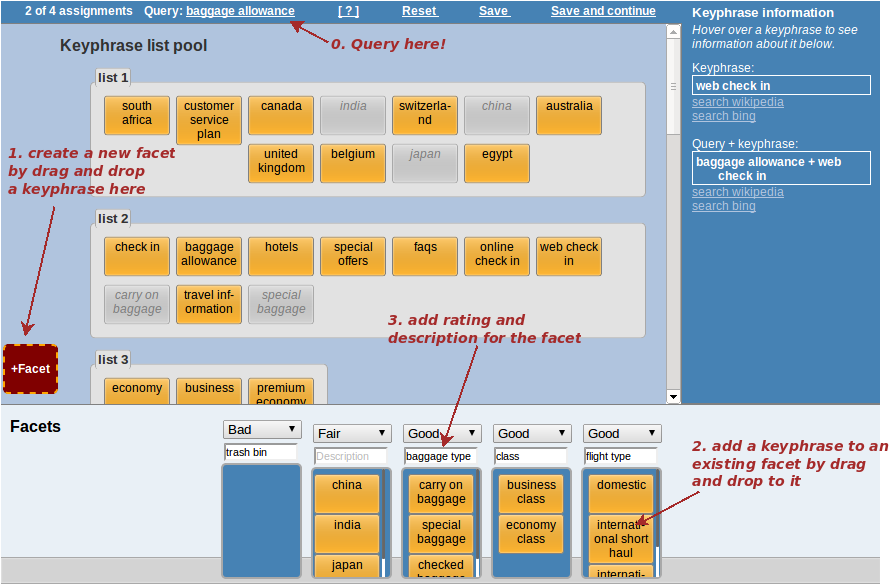
\epsfig{file=figure/facet-annotation-ui.png,scale=0.45}
%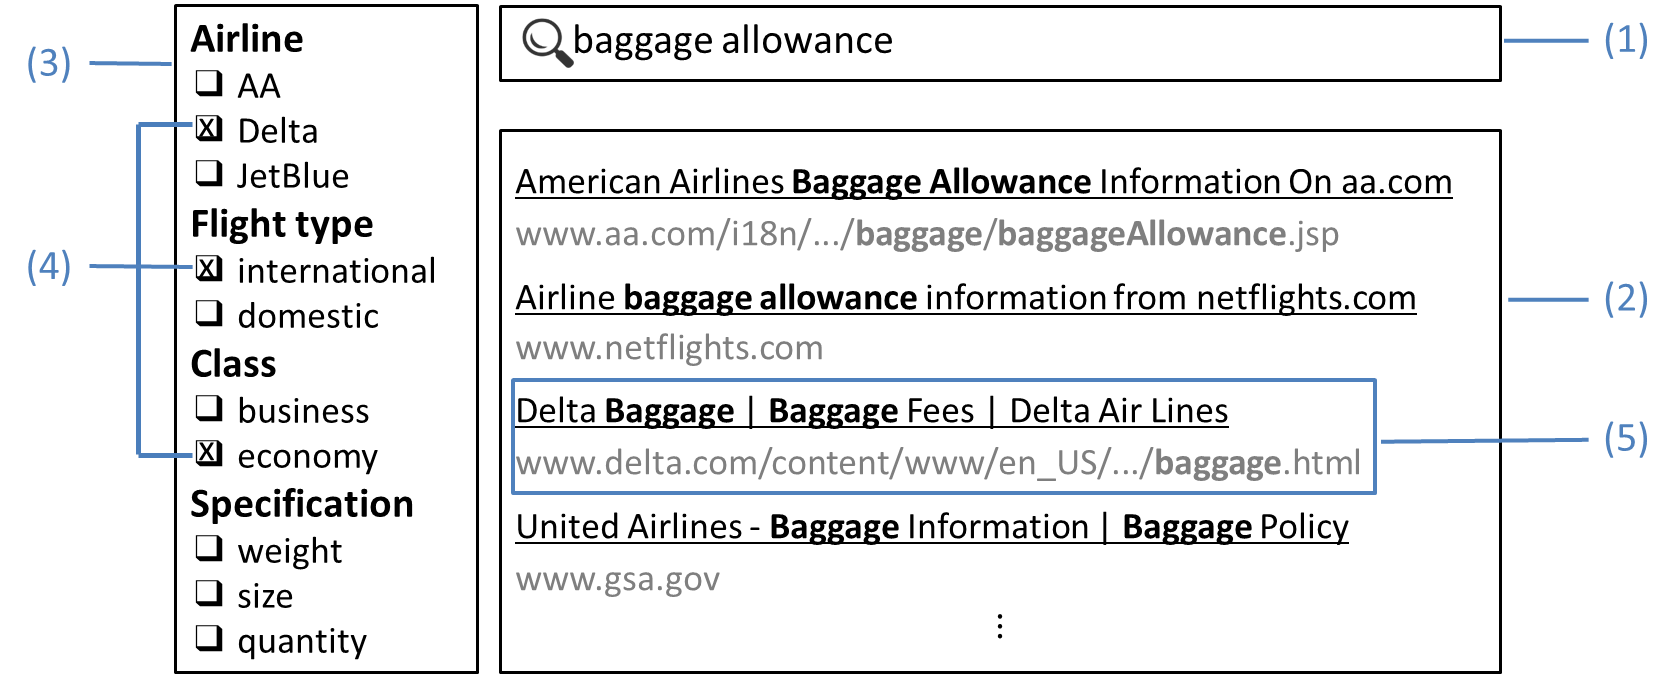
\includegraphics[scale=0.45]{figure/fws-example.png}
\caption{Annotation interface for query facet annotation.}
\label{fig:facet-annotation}
\end{figure}

\subsection{Query facet annotations}
\todo{include inter-annotator agreement on facts}
\todo{move annotation method in to an individual section, and talk about annotation trials.}
We asked human annotators to construct query facets as ground truth, using the annotation interface shown in Figure~\ref{fig:facet-annotation}.
For each query, we first constructed a pool of terms by aggregating facet terms in the top 10 query facets generated by different models (corresponding to ``keyphrase list pool'' in Figure~\ref{fig:facet-annotation}), including two runs from QDM, one run from each of pLSA and LDA using top 10 list items in each query facets, and one run for our graphical model based approach. 
Then, annotators were asked to group terms in the pool into query facets for each query they selected (corresponding to step 1 and 2 in Figure~\ref{fig:facet-annotation}).
Finally, the annotator was asked to give a rating for each constructed query facet, regarding how useful and important the query facet is (corresponding to step 3 in Figure~\ref{fig:facet-annotation}). The rating scale of good=2/fair=1 is used. 

We recruited 17 human annotators (5 females and 12 males), with 16 graduate students (computer science major) and 1 undergraduate student from our university. Prior to the actual annotation task, annotators were assigned a training session (using another query that is not in the data set) to get familiar with the task and annotation interface.

There are 50 query facets pooled per query, with 224.8 distinct facet terms per query. Annotation statistics for the good and fair facets, as well as the pooled facet, are given in Table~\ref{tab:annotations}. The table shows average number of facet terms per query, average number of query facets per query, and average number of facet terms per facet, for each categories (fair, good, and pooled facets).
\begin{table}[ht!]
\centering
\caption{Annotation statistics}
\label{tab:annotations}
\begin{tabular}{|l|r|r|r|} \hline
& fair & good & pooled\\ \hline
\#terms per query & 26.6 & 55.8 & 224.8\\ 
\#facets per query & 3.1 & 4.8 & 50.0 \\ 
\#terms per facet & 8.6 & 11.6 & 8.8 \\ \hline
\end{tabular}
\end{table}

\section{Metrics} 
\label{sec:ie-metrics}
Query facet extraction can be evaluated from different aspects. A good system should select ``correct'' facet terms from all the list items, therefore we use standard classification metrics, such as precision, recall and F-measures. A good system should also group those facet term correctly (i.e., in the same way as the annotators), therefore we use standard clustering metrics, such as F-measures for clustering, Purity and Normalized Mutual Information. To combine the different evaluation aspects, we design a new measure for this particular task.
\subsection{Notations} \label{sec:evalmetrics}
We continue to use notations defined in Section~\ref{sec:facet-formulation} for a query facet ($F$), a query facet set ($\mathcal{F}$) and the set of all facet terms ($T_{\mathcal{F}}$) in a query facet set. We use ``$*$'' to distinguish between system generated results and human labeled results, which we used as ground truth.
For example, $\mathcal{F}$ denotes the system generated query facet set, and $\mathcal{F}^*$ denotes the human labeled query facet set.
For convenience, we use $T$ to denote $T_{\mathcal{F}}$ in this Chapter, omitting subscript $\mathcal{F}$.
$T^*$ denotes all the facet terms in human labeled query facet set.
We use $r_{F^*}$ to denote the rating score for a human labeled facet $F^*$.

\subsection{Effectiveness in finding facet terms}
\label{sec:intrinsic-tmeasures}
One aspect of query facet extraction evaluation is how well a system finds facet terms. This can be evaluated using standard classification metrics as follows,
\begin{itemize}
 \item facet term precision: $T\!P=\frac{|T \cap T^*|}{|T|}$
 \item facet term recall: $T\!R=\frac{|T \cap T^*|}{|T^*|}$
 \item facet term F1: $T\!F=\frac{2|T \cap T^*|}{|T|+|T^*|}$
\end{itemize}
where the \concept{T} in measure names $T\!P$, $T\!R$, $T\!F$ stands for facet \emph{term}. It is used to distinguish the term based measures from term pair based measures as defined below. Note that these metrics do not take clustering quality into account.
%The system identified facet terms, $T$, are evaluated against human labeled ones, $T^*$, using Precision, Recall and F1.

\subsection{Clustering quality}
\label{sec:intrinsic-pmeasures}
To evaluate how well a system groups facet terms correctly,
similar to Dou et al.~\cite{dou2011finding}, we use several existing cluster metrics, namely, Purity, NMI/Normalized Mutual Information and pair-counting F1 measure. Here the pair-counting F1 measure treats term clustering as classification on whether each pairs of terms are in a same facet, and then combines pair precision and recall using F1 measure. We denote the pair-counting F1 measure as $P\!F$ with \concept{P} standing for term \emph{pair}.

%To avoid confusion with facet term F1, FT, we call F1 for facet term clustering \textit{facet clustering F1}, and denote it as FP (with \textit{P} standing for term \emph{pair}).

In our task, we usually have $T\neq T^*$. The facet terms in the system generated and human labeled clustering results might be different: the system might fail to include some human identified facet terms, or it might mistakenly include some ``incorrect'' facet terms. These standard clustering metrics cannot handle these cases properly. To solve this problem, we adjust $\mathcal{F}$ and $\mathcal{F}^*$ as if only facet terms in $T \cap T^{*}$ were clustered by the system, since we are only interested in how well the ``correct'' facet terms are clustered from these metrics. The adjusting is done by removing ``incorrect'' facet terms ($t \in T-T^*$) from $\mathcal{F}$, and removing missing facet terms ($t^{*}\in T^*-T$) in $\mathcal{F}^{*}$.  By this adjusting, we do not take into account the effectiveness of finding correct facet terms.

\subsection{Overall quality}
\label{sec:evalmetricsall}
\todo{more details, and re-structure}
To evaluate the overall quality of query facet extraction, Dou et al.~\cite{dou2011finding} proposed variations of nDCG (Normalized Discounted Cumulative Gain), namely purity aware nDCG (pNDCG, abbreviated as fp-nDCG in the original paper) and recall and purity aware nDCG (prNDCG, abbreviated as rp-nDCG in the original paper). They first map each system generated facet $F$ to a human labeled facet $F^*$ that covers the maximum number of terms in $F$. Then, they assign the rating $r_{F^*}$ to $F$, and evaluate $\mathcal{F}$ as a ranked list of query facets using nDCG.
The discounted gains are weighted by precision and/or recall of facet terms in $F$, against its mapped human labeled facet $F^*$. For \textbf{pNDCG}, only precision is used as weight, $\frac{|F^* \cap F|}{|F|}$.
For \textbf{prNDCG}, precision and recall are multiplied as weight, $\frac{|F^* \cap F|^2}{|F^*||F|}$. One other way is to use F1 for weighting as $\frac{2|F^* \cap F|}{|F^*| + |F|}$, and we call this measure \textbf{fNDCG}.

However, this these nDCG variation measures can be problematic in some cases.
When two facets $F_1$ and $F_2$ are mapped to a same human labeled facet $F^*$, only the first facet $F_1$ is credited and $F_2$ is simply ignored, even if it is more appropriate to map $F_2$ to $F^*$ (e.g., $F_2$ is exactly same as $F^*$, while $F_1$ contain only one facet term in $F^*$). Our proposed metric does not need to map facets, and thus does not have this problem.

The quality of query facet extraction is intrinsically multi-faceted. Different applications might have different emphasis in the three factors mentioned above - precision of facet terms, recall of facet terms 
and clustering quality of facet terms. We propose a metric $PRF_{\alpha,\beta}$ to combine the three factors together, using weighted harmonic mean, as follows

\begin{equation}
\label{eq:prf}
 P\!R\!F_{\alpha,\beta}(T\!P, T\!R, P\!F) = \frac{(\alpha^2 + \beta^2 + 1)}{\frac{\alpha^2}{T\!P} + \frac{\beta^2}{T\!R} + \frac{1}{P\!F}},
\end{equation}
where $\alpha,\beta \in [0,+\infty)$ are used to control the weight between the three factors in the same way as ``$\beta$'' in F-measures~\cite{van1979information}. $\alpha$ and $\beta$ can be interpreted as the importance of $T\!P$ and $T\!R$ compared to $P\!F$ respectively. More formally, we have 
\begin{equation}
\begin{split} 
 when\; \alpha &= \frac{T\!P}{P\!F} \;, \frac{\partial P\!R\!F_{\alpha,\beta}}{\partial T\!P} = \frac{\partial P\!R\!F_{\alpha,\beta}}{\partial P\!F}\\
 when\; \beta &= \frac{P\!R}{P\!F} \;, \frac{\partial P\!R\!F_{\alpha,\beta}}{\partial T\!R} = \frac{\partial P\!R\!F_{\alpha,\beta}}{\partial P\!F}.
\end{split}
\end{equation}
The intuition behind this is we want to specify the $T\!P/P\!F$ ratio at which the user is willing to trade an increment in $T\!P$ for an equal loss in $P\!F$, and similarly for $T\!R/P\!F$. For example, we can set $\alpha\!=\!2,\beta\!=\!1$ to evaluate the case where $T\!P$ is twice important than $T\!R$ and $P\!F$. When $\alpha \!=\! \beta \!=\! 1$, we omit the subscript part for simplicity, i.e. $PRF \equiv PRF_{1,1}$.

While $PRF_{\alpha,\beta}$ has the flexibility to adjust emphasis between the three factors, it does not take into account the different ratings associated with query facets. To incorporate ratings, we use a weighted version of $T\!P$, $T\!R$ and $P\!F$ in $PRF_{\alpha,\beta}$. We call the new metric $wPRF_{\alpha,\beta}$. The weighted facet term precision, recall and $T\!F$ are defined as follows.
\begin{itemize}
 \item weighted facet term precision: $wT\!P=\frac{\sum_{t \in T \cap T^*}{w(t)}}{\sum_{t \in T}{w(t)}}$
 \item weighted facet term recall: $wT\!R=\frac{\sum_{t \in T \cap T^*}{w(t)}}{\sum_{t^* \in T^*}{w(t^*)}}$ 
  \item weighted facet term F1: $wT\!F=\frac{2wP(T,T^*)wR(T,T^*)}{wP(T,T^*)+wR(T,T^*)}$ 
\end{itemize}
where $w(t)$ is the weight for facet term $t$, and assigned as follows
$$
w(t) = \left\{ \begin{array}{rl}
r_{F^*} &\mbox{ if $t \in T^*$} \\
1 &\mbox{ otherwise}
\end{array} \right.
$$
Similarly, $wP\!F$ is computed by weighting its pairwise precision and recall in the same fashion as the weighted facet term precision and recall above.
Instead of $w(t)$, we need weight for a pair of facet terms $w(t_1,t_2)$ in this calculation.
We assign weight for facet term pair $w(t_1, t_2)$ using their sum, $w(t_1) + w(t_2)$.


\section{Experiments}
\label{sec:ie-exp}
\todo{Need an introduction}
\todo{Some results need to be updated}
\todo{add more experiments testing extraction patterns, features}
\subsection{Experiment settings}
\todo{separate to multiple paragraphs}
We compare effectiveness of the five models, QDM, pLSA, LDA and QFI, QFJ (described in Chapter~\ref{ch:facet}), on the 100-query data set.
All the models take the same candidate lists extracted/cleaned (see Section~\ref{sec:facet-candidate}) as input.
We perform 10-fold cross validation for training/testing and parameter tuning in all experiments and for all models (if applicable).
When training the graphical model, we standardize features by removing the mean and scaling to unit variance.
We set both of the two regularizers $\sigma$ and $\gamma$ to be 1.
%we use logistic regression implemented in scikit-learn~\cite{scikit-learn} to estimate $\mu$ and $\lambda$ in Equation~\ref{eq:lg}, and set both regularizers $\sigma$ and $\gamma$ to be 1.
There are too many negative instances ($y_i=0$, $z_{i,j}=0$) in the training data, so we stratify samples by labels with the ratio of positive:negative to be 1:3.
For QDM, we tune the two parameters used in the clustering algorithm $Dia_{max}$ (the diameter threshold for a cluster) and $W_{min}$ (the weight threshold for a valid cluster), as well as two parameters used for selecting facet terms in each facet ($S_{t|F} > \alpha |Sites(F)|$ and $S_{t|F}>\beta$).
%QDM selects facet terms as output for each query facet, when the query facets meets both of the following conditions: $S_{t|F} > \alpha |Sites(F)|$ and $S_{t|F}>1$, where $S_{t|F}$ is a score for facet term $t$, and $Sites(F)$ is the set of websites that contains any of the candidate lists in query facet $F$.
%We also tune the parameter $\alpha \in \{0, 0.02, 0.04, 0.06, 0.08, 0.1, 0.12\}$.
%Since the second condition may also prevent QDM from showing more facet term in a query facet, we also tried to exclude this condition, and tune $\alpha \in \{0, 0.005, 0.01, 0.015, 0.02\}$ in this case.
For pLSA and LDA, we tune the number of facet terms in a query facet.
% $n \in \{5, 8, 10, 11, 12, 13, 14, 15, 16, 17, 18, 19, 20\}$.
%_\{0.4, 0.5, 0.6, 0.7, 0.8\}$
For QFI, we tune the weight threshold for facet terms, $w_{min}$, and the diameter threshold,  $d_{max}$.
%\in \{0.5, 0.6, 0.7\}
For QFJ, there are no parameter need to be tuned.
We returned top 10 query facets from all the five models in all evaluation. 
\subsection{Finding Facet Terms}
\label{sec:expt}
We first evaluate the models in terms of their effectiveness in finding facet terms, using classification measures described in Section~\ref{sec:intrinsic-tmeasures}. More specifically, we compare the classification performance of these models in terms of term precision (TF), term recall (TR), term F1 (TF) and their weighted versions (wTF, wTR, wTF). We compare results tuned on TF, which keeps a balance between term precision and term recall, and wTF, which, in addition, takes facet term weighting into account.


We report the results in Table~\ref{tab:intrinsic-tf}. From the table, we can see that QFI and QFJ perform relatively well for both precision and recall. Their improvements over the other three models shown are all statistically significant (p < 0.05, using paired t-test) \todo{need to test}. The two topic model based approaches, pLSA and LDA, have relatively high recall and low precision. Contrarily, QDM has higher precision than the two topic models, but low recall.
This difference can be explain by the number of face terms each model returned, as shown in the last column of the table. QDM only outputs 93.4 facet terms per query, while pLSA and LDA both output much more facet terms. One possible reason for the low precision of pLSA and LDA is that they select facet terms solely according to term probabilities in the learned topics (query facets in our case) and do not explicitly incorporate query relevance. We find most of their facet terms are frequently-occurring list items, which are not necessary relevant to the query.
While the numbers of facet terms QFI and QFJ output are similar to QDM, QFI and QFJ obtain much higher precision and recall, likely due to the rich set of features used, which captures both how likely a list item is a coordinate term, and how its relevance to the query. We will analyze these features in later sections \todo{add ref}. 

\begin{table}[ht!]
\centering
\caption{Facet term classification performance. Results in the upper part are tuned on TF, and results in the bottom part are tuned on wTF. ``\#terms'' shows the average number of facet terms returned per query for each models. The best performance scores are marked in boldface.}
\label{tab:intrinsic-tf}
\begin{tabular}{|c|c|c|c|c|c|c|r|} \hline
\multicolumn{8}{|c|}{Tuned on TF} \\\hline
model& TP & TR & TF & wTP & wTR & wTF & \#terms \\ \hline
QDM & 0.3124 & 0.3182 & 0.2926 & 0.2773 & 0.2852 & 0.2604 & 93.4 \\\hline
pLSA & 0.2627 & \textbf{0.5640} & 0.3350 & 0.2305 & 0.5001 & 0.2950 & 175.0 \\ \hline
LDA & 0.2743 & 0.5382 & 0.3365 & 0.2385 & 0.4743 & 0.2941 & 154.0 \\ \hline
QFJ & 0.3986 & 0.4832 & 0.4161 & 0.3482 & 0.4267 & 0.3650 & 97.0 \\ \hline
QFI & \textbf{0.4157} & 0.5543 & \textbf{0.4472} & \textbf{0.3712} & \textbf{0.5018} & \textbf{0.4017} & 107.9 \\ 
\hhline{|========|}
\multicolumn{8}{|c|}{Tuned on wTF} \\\hline
model& TP & TR & TF & wTP & wTR & wTF & \#terms \\ \hline
QDM & 0.3124 & 0.3182 & 0.2926 & 0.2773 & 0.2852 & 0.2604 & 93.4 \\ \hline
pLSA & 0.2627 & 0.5640 & 0.3350 & 0.2305 & 0.5001 & 0.2950 & 175.0 \\ \hline
LDA & 0.2625 & \textbf{0.5936} & 0.3389 & 0.2301 & \textbf{0.5285} & 0.2988 & 180.0 \\ \hline
QFJ & 0.3986 & 0.4832 & 0.4161 & 0.3482 & 0.4267 & 0.3650 & 97.0 \\ \hline
QFI & \textbf{0.4058} & 0.5670 & \textbf{0.4461} & \textbf{0.3623} & 0.5126 & \textbf{0.4003} & 112.6 \\ \hline
\end{tabular}
\end{table}

From Table~\ref{tab:intrinsic-tf}, we also find the the weighted measures are usually consistent with their corresponding unweighted measures.
%One exception is that QFJ performs better than QFI in FT, but it does slightly worse than QFJ in wFT. This is likely to be caused by the high recall for QFI, which may include more highly rated facet terms.

\subsection{Clustering Facet Terms}
Next, we evaluate the models in terms of their effectiveness in clustering facet terms, using clustering measures described in Section~\ref{sec:intrinsic-pmeasures}. More specifically, we compare the clustering performance of these models in terms of pair counting F1 (PF), wPF (weighted version of PF), Purity and NMI (Normalized Mutual Information). We compare results tuned on PF  and wPF, which takes facet term weighting into account.

We report the results in Table~\ref{tab:intrinsic-pair}. From the table, we can see that QFI and QFJ perform relatively well for PF, wPF and NMI. The improvements of QFI and QFJ over the other three models shown are all significant (p < 0.05, using paired t-test)\todo{test}. For purity, pLSA and LDA obtain relatively higher score, which is due to that they returned relatively small number of facet terms (shown in ``\#terms'' fields), and thus only cluster a very small number of terms together in each clusters.  These observations are consistent for the runs tuned on PF and its weighted version, wPF.

%Contrarily, pLSA and LDA do not perform for other clustering measures. well in clustering, which could be caused by data sparsity. There are on average 5159 candidate lists per query, but only 3.9 items per list. 

\begin{table}[ht!]
\centering
\caption{Facet term clustering performance. Results in the upper part are tuned on PF, and results in the bottom part are tuned on wPF. We also report corresponding classification performance in the left part using term precision (TP), term recal (TR) and term F1 (TF). ``\#terms'' shows the average number of facet terms returned per query for each models. The best performance scores are marked in boldface.}
\label{tab:intrinsic-pair}
\begin{tabular}{|c|c|c|c|c||c|c|c|r|} \hline
\multicolumn{9}{|c|}{Tuned on PF} \\\hline
Model & PF & wPF & Purity & NMI & TP & TR & TF & \#terms \\ \hline
QDM & 0.5543 & 0.5435 & 0.9484 & 0.5734 & 0.2489 & 0.2628 & 0.2206 & 103.9 \\ \hline
pLSA & 0.4270 & 0.4119 & \textbf{0.9746} & 0.5643 & 0.3355 & 0.1255 & 0.1646 & 28.9 \\ \hline
LDA & 0.3860 & 0.3657 & 0.9672 & 0.5616 & 0.3492 & 0.1388 & 0.1797 & 30.0 \\ \hline
QFJ & 0.6961 & 0.6633 & 0.9346 & 0.6285 & \textbf{0.3986} & \textbf{0.4832} & \textbf{0.4161} & 97.0 \\ \hline
QFI & \textbf{0.7397} & \textbf{0.7130} & 0.9628 & \textbf{0.6336} & 0.2063 & 0.4052 & 0.2592 & 161.5 \\ 
\hhline{|=========|}
\multicolumn{9}{|c|}{Tuned on wPF} \\\hline
Model & PF & wPF & Purity & NMI & TP & TR & TF & \#terms \\ \hline
QDM & 0.5831 & 0.5751 & 0.9772 & 0.5776 & 0.2236 & 0.1763 & 0.1636 & 92.7 \\ \hline
pLSA & 0.4327 & 0.4223 & \textbf{0.9845} & 0.5673 & 0.3398 & 0.0993 & 0.1437 & 21.8 \\ \hline
LDA & 0.4176 & 0.4007 & 0.9775 & 0.5646 & 0.3595 & 0.1132 & 0.1575 & 23.4 \\ \hline
QFJ & 0.6961 & 0.6633 & 0.9346 & 0.6285 & \textbf{0.3986} & \textbf{0.4832} & \textbf{0.4161} & 97.0 \\ \hline
QFI & \textbf{0.7370} & \textbf{0.7090} & 0.9635 & \textbf{0.6325} & 0.2055 & 0.3993 & 0.2570 & 159.5 \\ \hline
\end{tabular}
\end{table}


The better performance in clustering for QFI and QFJ can be explained by their incorporating factors other than list item co-occurrence information. In our feature analysis (in later sections \todo{add ref}), besides one item co-occurrence related feature, \textit{listContextSim}, we also find that \textit{textContextSim} has a relatively high weight. \textit{textContextSim} is used to capture the similarity of the two list items using their surrounding text, so it can help to group two facet terms together even if they might not co-occur a lot in candidate lists. As an example, for the query \textit{baggage allowance}, we find different airlines do not co-occur a lot in candidate lists, (e.g. \textit{delta} and \textit{jetblue} only co-occur twice), but they tend to have high \textit{textContextSim} (e.g. $TextContextSim(delta,jetblue)=0.81$), and are therefore grouped together by QFI and QFJ \todo{check}.

From Table~\ref{tab:intrinsic-pair}, we also find term clustering performance does not necessarily ``agree'' with term classification performance. Comparing QFI and QFJ, we find QFI obtains better clustering performance of the facet terms it selected, but does relatively poorly in selecting facet terms. Thus, next we will investigate the overall performance.


\subsection{Overall Evaluation}
To compare overall effectiveness of the five models, in this section, we focus on using \PRF measure with equal weight between term precision, term recall and term clustering (denoted as PRF). We will investigate unbalanced weighting in \PRF in Chapter~\ref{ch:precision}.


We tune all the models on PRF, as well as its weighted version (wPRF). We report the overall measure scores (PRF, wPRF), as well as its constituent factors (TP, TR, PF and wTP, wTR, wPF), in order to see the details. We also report the rank measures, pNDCG, prNDCG and fNDCG, to see if whether PRF based measures agree with these ranking measures. The results are given in Table~\ref{tab:intrinsic-all}.

\begin{table}[ht!]
\centering
\caption{Overall performance tuned on PRF (upper) and wPRF (bottom). We also include term precision (TP), term recall (TR), term clustering pair counting F1 (PF), and their weighted versions (wTP, wTR and wPF). We also report ranking-based measures pNDCG, prNDCG and fNDCG, which weight the DCG gains by purity (or precision), recall and F1 of facet terms respectively. The best performance scores are marked in boldface.}
\label{tab:intrinsic-all}
\begin{tabular}{|c|c|c|c|c|c|c|c|r|} \hline
\multicolumn{9}{|c|}{Tuned on PRF} \\\hline
Model & TP & TR & PF & PRF & pNDCG & prNDCG & fNDCG & \#terms \\ \hline
QDM & 0.2946 & 0.3284 & 0.5662 & 0.3279 & 0.1554 & 0.0564 & 0.1441 & 102.5 \\ \hline
pLSA & 0.2744 & \textbf{0.5027} & 0.4372 & 0.3411 & 0.1294 & 0.0508 & 0.1439 & 148.0 \\ \hline
LDA & 0.2802 & 0.4975 & 0.4018 & 0.3293 & 0.1307 & 0.0496 & 0.1411 & 138.6 \\ \hline
QFJ & 0.3986 & 0.4832 & \textbf{0.6961} & 0.4654 & \textbf{0.3256} & \textbf{0.1771} & \textbf{0.2946} & 97.0 \\ \hline
QFI & \textbf{0.4450} & 0\.4881 & 0.6209 & \textbf{0.4720} & 0.3176 & 0.1626 & 0.2857 & 89.5 \\ 
\hhline{|=========|}
\multicolumn{9}{|c|}{Tuned on wPRF} \\\hline
Model & wTP & wTR & wPF & wPRF & pNDCG & prNDCG & fNDCG & \#terms \\ \hline
QDM & 0.2572 & 0.2967 & 0.5435 & 0.2941 & 0.1538 & 0.0565 & 0.1441 & 104.9 \\ \hline
pLSA & 0.2305 & 0.5001 & 0.3998 & 0.3062 & 0.1082 & 0.0500 & 0.1363 & 175.0 \\ \hline
LDA & 0.2287 & \textbf{0.5276} & 0.3686 & 0.2955 & 0.1065 & 0.0485 & 0.1298 & 180.0 \\ \hline
QFJ & 0.3482 & 0.4267 & \textbf{0.6633} & 0.4144 & \textbf{0.3256} & \textbf{0.1771} & \textbf{0.2946} & 97.0 \\ \hline
QFI & \textbf{0.3897} & 0.4420 & 0.5891 & \textbf{0.4263} & 0.3167 & 0.1627 & 0.2858 & 90.6 \\ \hline
\end{tabular}
\end{table}

Results in Table~\ref{tab:intrinsic-all} are mostly consistent with the results that were tuned on FT and TF (and their weighted version) in the classification and clustering evaluation above. QDM obtain relatively low term precision and low term recall, but better clustering performance on the selected facet terms (PF and wPF). pLSA and LDA have high recall, but low precision and PF/wPF. This is due to that pLSA and LDA return a lot of facet terms. There are on average 81.15 facet terms per query for the human annotated query facets, but pLSA and LDA returned around twice of the amount. QFI and QFJ are the best two models according to the overall performance measures, PRF, wPRF and pNDCG, prNDCG, fNDCG. The differences are statistically significant (p < 0.05 based on paired t-test). We will analysis more on QFI's and QFJ's success in future sections (\todo{add ref}).

Comparing the results tuned on PRF and its weighted version, wPRF, we find weighting encourages returning more facet terms slightly, which is shown in the field \concept{\#terms}, the average number of facet terms returned per query. This can be explained by that returning more terms may increase the number of high-rating facet terms found, and thus increase wPRF.\todo{investigation of weighted measures.} Comparing the results for PRF, wPRF with the results for pNDCG, prNDCG, fNDCG, we find the two types of measures agree with each other in general (\eg, QFJ and QFI are better than other three models), but not always (QFI is better than QFJ for the PRF measures, but worse than QFJ for the NDCG measures). 


Since PRF/wPRF do not always agree with the ranking-based measures, and PRF/wPRF do not account for facet ranking effectiveness, we also test the models based on results tuned on these ranking-based measures. We report results for the ranking-based measures and PRF/wPRF tuned on fNDCG in Table~\ref{tab:intrinsic-rank} (results tuned on pNDCG, prNDCG are similar). 
QFI and QFJ are the best two models for the ranking-based measures. QFJ gives the best performance for prNDCG and fNDCG, which combine both precision and recall of facet terms in weighting DCG. These observations are consistent with the results tuned on PRF/wPRF in Table~\ref{tab:intrinsic-all}. 
\todo{add t-test}
%The improvements of QFI and QFJ over the other three models shown are significant (p < 0.05, using paired t-test), except the improvements of QFJ over QDM for wP and QFI over QDM for fp-nDCG.

\begin{table}[h!]
\centering
\caption{fp-nDCG and rp-nDCG tuned on themselves}
\label{tab:intrinsic-rank}
\begin{tabular}{|c|c|c|c|c|c|r|} \hline
Model & pNDCG & prNDCG & fNDCG & PRF & wPRF & \#terms \\ \hline
QDM & 0.1442 & 0.0550 & 0.1410 & 0.3331 & 0.2991 & 113.4 \\ \hline
pLSA & 0.1838 & 0.0674 & 0.1756 & 0.3303 & 0.2880 & 139.0 \\ \hline
LDA & 0.1718 & 0.0594 & 0.1588 & 0.3259 & 0.2844 & 145.5 \\ \hline
QFJ & 0.3256 & \textbf{0.1771} & \textbf{0.2946} & 0.4654 & 0.4144 & 97.0 \\ \hline
QFI & \textbf{0.3350} & 0.1618 & 0.2825 & \textbf{0.4678} & \textbf{0.4197} & 77.5 \\ \hline
\end{tabular}
\end{table}

\subsection{Feature Analysis}
In our analysis above, we credit the success of QFI/QFJ models to the rich set of features they used. In this section, we analyze these features to (1) test our hypothesis that the success of QFI/QFJ is due to the rich set of features and (2) discovery which features are important and which are not.

We first test the importance of our features by their weight learned in the model. Note that our features has been standardized (removing the mean and scaling to unit variance), and thus the weights are comparable. Higher weight in its absolute suggests the corresponding feature is more important. Table~\ref{tab:intrinsic-tanalysis} shows the weight learned for item features (Section~\ref{sec:facet-features}) in one fold of the 10-fold cross-validation (results are similar for other folds). Not surprisingly, list TF/IDF based features which are used to capture the likelihood of being a coordinate term have relatively high weights, with \textit{ListTermFreq.ListIDF} being the most important features. Other features that are used to capture query relevance also obtain relatively high weight, \eg, \textit{ContentSiteFreq}, \textit{ContentTermFreq.IDF}. 
%We also find features that are relatively less important. 
\begin{table}[H]
\centering
\caption{Item feature weights learned in one fold of the 10-fold cross-validation (results are similar for other folds). Features are sorted by the absolute value of the weights. The features are explained in Table~\ref{tab:facet-tfeature}.}
\label{tab:intrinsic-tanalysis}
\begin{tabular}{|r|r|} \hline
Feature & Weight \\ \hline
ListTermFreq.ListIDF & 2.1620 \\ \hline
ListSelectSiteFreq & 1.9604 \\ \hline
ContentSiteFreq & 1.5251 \\ \hline
ListTextSiteFreq & 1.3860 \\ \hline
ListSelectPageFreq & -1.0627 \\ \hline
ListTrTermFreq & -0.8608 \\ \hline
ListTdPageFreq & -0.8248 \\ \hline
ContentTermFreq.IDF & 0.8195 \\ \hline
ContentWPageFreq & -0.7475 \\ \hline
ListTrSiteFreq & 0.7438 \\ \hline
ListIDF & -0.6863 \\ \hline
ListTdSiteFreq & 0.6491 \\ \hline
IDF & -0.6207 \\ \hline
ListTextPageFreq & -0.5431 \\ \hline
ContentPageFreq & 0.4560 \\ \hline
ContentTermFreq & -0.4193 \\ \hline
ListUlPageFreq & 0.2985 \\ \hline
ListSelectTermFreq & -0.2908 \\ \hline
ListTdTermFreq & 0.2740 \\ \hline
Length & -0.2615 \\ \hline
TitleTermFreq & 0.2497 \\ \hline
ListUlSiteFreq & 0.2438 \\ \hline
ListUlTermFreq & -0.2345 \\ \hline
ListOlSiteFreq & -0.1507 \\ \hline
TitleSiteFreq & -0.1271 \\ \hline
ListOlTermFreq & 0.1203 \\ \hline
ListOlPageFreq & 0.1076 \\ \hline
TitlePageFreq & -0.0447 \\ \hline
ListTrPageFreq & -0.0424 \\ \hline
ListTextTermFreq & -0.0295 \\ \hline
\end{tabular}
\end{table}

In Table~\ref{tab:intrinsic-panalysis}, we show the weights learned for item pair feature (Section~\ref{sec:facet-features}) in one fold of the 10-fold cross-validation (results are similar for other folds). The table suggests that \textit{ContextListSim} and \textit{ContextTextSim} are the two most important item pair features. Though both \textit{ContextListSim} and \textit{ListCooccur} are based on the item occurrence in candidate lists, the weight for \textit{ListCooccur} is far less than the weight for \textit{ContextListSim}. This can be explained by the example in Table~\ref{tab:facet-listcontext}, which shows that \textit{ContextListSim} can assign high value for semantically related list items, even if they do not co-occur in a candidate list.

\begin{table}[H]
\centering
\caption{Item pair feature weights learned in one fold of the 10-fold cross-validation (results are similar for other folds). Features are sorted by the absolute value of the weights. The features are explained in Table~\ref{tab:facet-pfeature}.}
\label{tab:intrinsic-panalysis}
\begin{tabular}{|r|r|} \hline
Feature & Weight \\ \hline
ContextListSim & 1.5373 \\ \hline
ContextTextSim & 0.7754 \\ \hline
ListCooccur & 0.0643 \\ \hline
LengthDiff & 0.0271 \\ \hline
\end{tabular}
\end{table}

Next we investigate the effectiveness of our features based on feature ablation experiments, in which we remove one feature (or a set of features) at a time to examine the effectiveness of the each feature (or feature set) in the presence of other features. The results are reported in Table~\ref{tab:intrinsic-ablation}.
\begin{table}[H]
\centering
\caption{PRF performance changes when suppressing each features or feature sets. $\Delta$PRF shows the PRF performance change when excluding the corresponding feature (or feature set). $\Delta$PRF\% shows the PRF change in percentage. ListText, ListUl, ListSelect, ListOl, ListTr, ListTd, Content, Title denote feature sets in which the features are extracted from the corresponding fields (\eg, ListText = \{ListTextTermFreq, ListTextPageFreq, ListTextSiteFreq\}). 
%\textit{List} denote features extracted from all types candidate lists. 
The results are based on QFJ model tuned on PRF (other results are similar).}
\label{tab:intrinsic-ablation}
\begin{tabular}{|r|r|r|r|} \hline
Feature/Feature set & PRF & $\Delta$PRF & $\Delta$PRF\% \\ \hline
%List & 0.4305 & -0.0349 & -7.50\% \\ \hline
ContextListSim & 0.4416 & -0.0238 & -5.11\% \\ \hline
ListText & 0.4454 & -0.0200 & -4.30\% \\ \hline
ListTermFreq.ListIDF & 0.4465 & -0.0189 & -4.06\% \\ \hline
ContextTextSim & 0.4531 & -0.0123 & -2.64\% \\ \hline
ListUl & 0.4599 & -0.0055 & -1.18\% \\ \hline
ListSelect & 0.4615 & -0.0039 & -0.84\% \\ \hline
LengthDiff & 0.4616 & -0.0038 & -0.82\% \\ \hline
IDF & 0.4620 & -0.0034 & -0.73\% \\ \hline
Content & 0.4621 & -0.0033 & -0.71\% \\ \hline
ListTd & 0.4633 & -0.0021 & -0.45\% \\ \hline
ListTr & 0.4635 & -0.0019 & -0.41\% \\ \hline
Title & 0.4638 & -0.0016 & -0.34\% \\ \hline
Length & 0.4643 & -0.0011 & -0.24\% \\ \hline
ListIDF & 0.4650 & -0.0004 & -0.09\% \\ \hline
ListCooccur & 0.4653 & -0.0001 & -0.02\% \\ \hline
ContentTermFreq.IDF & 0.4657 & 0.0003 & 0.06\% \\ \hline
ListOl & 0.4660 & 0.0006 & 0.13\% \\ \hline
\end{tabular}
\end{table}

From Table~\ref{tab:intrinsic-ablation}, we can see that the feature ablation experiments are in general consistent with our previous analysis based on feature weights. \textit{ContextListSim}, \textit{ListText} based features, \textit{ListTF.ListIDF}, \textit{ContextTextSim} are the most informative features. Comparing the feature sets ListText, ListUl ListSelect, ListTd, ListTr, ListOl, we find features based on candidate lists extracted from TEXT, UL and SELECT patterns are more informative. In the next section, we will further investigate these different extraction patterns.

\todo{experiment excluding more and more features}

\subsection{Comparing Extraction Patterns}
Similar as the feature ablation experiments, we investigate the effectiveness of different candidate list extraction patterns (Section~\ref{sec:facet-candidate}) by removing one extraction pattern at a time. Note this pattern ablation not only removes the candidate lists we used for refining facets, but also will affect the features we used in QFI and QFJ. For example, when excluding SELECT pattern, feature \textit{ListSelectTermFreq} will also be excluded. We report the results for QFI tuned on PRF in Table~\ref{tab:intrinsic-clists}.
\begin{table}[H]
\centering
\caption{PRF performance changes when suppressing each candidate list extraction pattern. $\Delta$PRF shows the PRF performance change when excluding the corresponding extraction pattern. $\Delta$PRF\% shows the PRF change in percentage. These patterns are explained in Section~\ref{sec:facet-candidate}). The results are based on QFI model tuned on PRF (other results are similar).}
\label{tab:intrinsic-clists}
\begin{tabular}{|r|r|r|r|} \hline
Pattern & PRF & $\Delta$PRF & $\Delta$PRF\% \\ \hline
Lexical & 0.3927 & -0.0793 & -16.80\% \\ \hline
UL & 0.4268 & -0.0452 & -9.58\% \\ \hline
SELECT & 0.4378 & -0.0342 & -7.25\% \\ \hline
TD & 0.4676 & -0.0044 & -0.93\% \\ \hline
TR & 0.4705 & -0.0015 & -0.32\% \\ \hline
OL & 0.4724 & 0.0004 & 0.08\% \\ \hline
\end{tabular}
\end{table}
From Table~\ref{tab:intrinsic-clists}, we can see that the lexical pattern plays a very importance role in query facet extraction. When excluding this lexical pattern, the PRF performance drop 16.80\%. Other important patterns are UL and SELECT. On the contrary, the patterns based on tables (TD, TR) and ordered list (OL) are found less important -- excluding them does not affect the results very much.

\todo{additional analysis of candidate lists: number, percentage of different list types, coverage over the query facets/terms. Global statistics.}

\section{Summary} \label{sec:ie-conclusions}
In this chapter, we designed intrinsic evaluation to directly evaluate generated query facets by comparing them with human created ones. We described how to collect human annotations for query facets as ground truth. We designed an evaluation measure that combines recall and precision of facet terms with grouping quality. We use this intrinsic evaluation to compare different query facet extraction models. Experimental results show that our supervised methods (QFI/QFJ), described in Chapter~\ref{ch:facet}, can take advantage of a richer set of features and outperforms other unsupervised methods. Our feature analysis suggests several informative features for query facet extraction, including \textit{ContextListSim}, \textit{ListTF.ListIDF}, \textit{ContextTextSim} and \textit{ListTextSiteFreq}. Our analysis on the candidate extraction patterns shows that the lexical pattern, UL pattern and SELECT patterns are more important than other patterns.


One thing we note is that term precision tends to be low while term recall is relatively high in these results. In the next chapter, we explore methods for boosting precision on the assumption that it is often more important.

